\documentclass[a4paper,10pt]{article}
\usepackage[english]{babel}
\usepackage[utf8]{inputenc}
\usepackage{graphicx}
\usepackage{amsmath,amssymb}
\usepackage{hyperref, url}
\usepackage{listings}
\usepackage[multiple]{footmisc}
\usepackage[english]{babel}
\usepackage{float}
\parindent 0mm
\parskip 3mm

% add your name and student number in parenthesis
\title{ICS-E4020: Week 2 - Correlated pairs}
\author{Néstor Castillo García (472081)\\ 
       {\tt nestor.castillogarcia@aalto.fi}}
\begin{document}

\maketitle

\section{Correlated Pairs}

\subsection{Description}

In this task, m input vectors with n numbers are given. The correlations between all pairs of input vectors is calculated. A red pixel at (i, j) indicates a positive correlation between vectos i and j, and a blue pixel indicates a negative correlation. The correlation coefficient r can be calculated in the following way.

\begin{equation} \label{eq:pcaErrorc}
 SS_{xx} = \sum x^2 - n\bar{x}^2
 \end{equation} 

\begin{equation} \label{eq:pcaErrorc}
  SS_{yy} = \sum y^2 - n\bar{y}^2
\end{equation} 

\begin{equation} \label{eq:pcaErrorc}
 SS_{xy} = \sum xy - n\bar{x}bar{y}
\end{equation} 

\begin{equation} \label{eq:pcaErrorc}
 r^2 = \frac{ss_{xy}^2}{ss_{xx}ss_{yy}}
\end{equation} 


\subsection{Implementation}
For practical and efficiency reasons. The previous calculations were simplified by  normalizing the input matix such that each the sum of squares in each row was one and its mean zero. Such normalization simplifies the correlation coefficient and the calculation is simplified to the following equation.

\begin{equation} \label{eq:pcaErrorc}
 r^2 = \sum xy 
\end{equation} 

\subsection{Hardware}
The computers had the following specifications: Intel Xeon E3-1230v2, 4 cores, 8 thread, 3,3 GHz, RAM: 16 GB, GPU: Nvidia K2000.

\subsection{Performance}
The computationally intensive part of the correlation image is the dot product, that in the vector solution was efficiently improved by using AVX operations. The matrix normalization is done in O(n) time. 

As expected, performance increased with the number of threads. The multithreded version was in average 2,6 times faster than the single threaded solution for the non vectorized code (CP2). In contrast, the multithreaded version of the vectorized code (CP3) was 4,9 times faster than the single threaded vectorized version.

\begin{figure}[H]
\centering
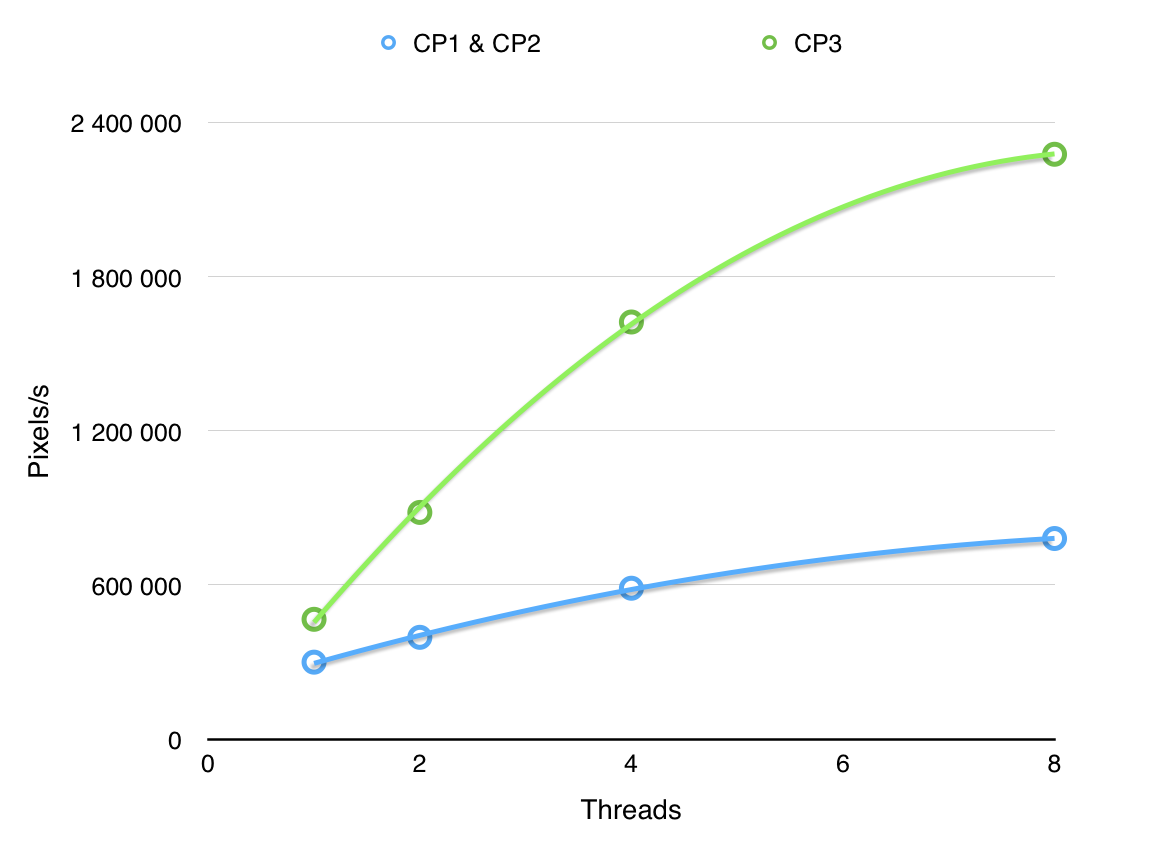
\includegraphics[width=1\textwidth]{figures/w2_pixels}
\caption{Pixels per second in a 4000 x 4000 image}
\label{fig:pca_type}
\end{figure}

\begin{figure}[H]
\centering
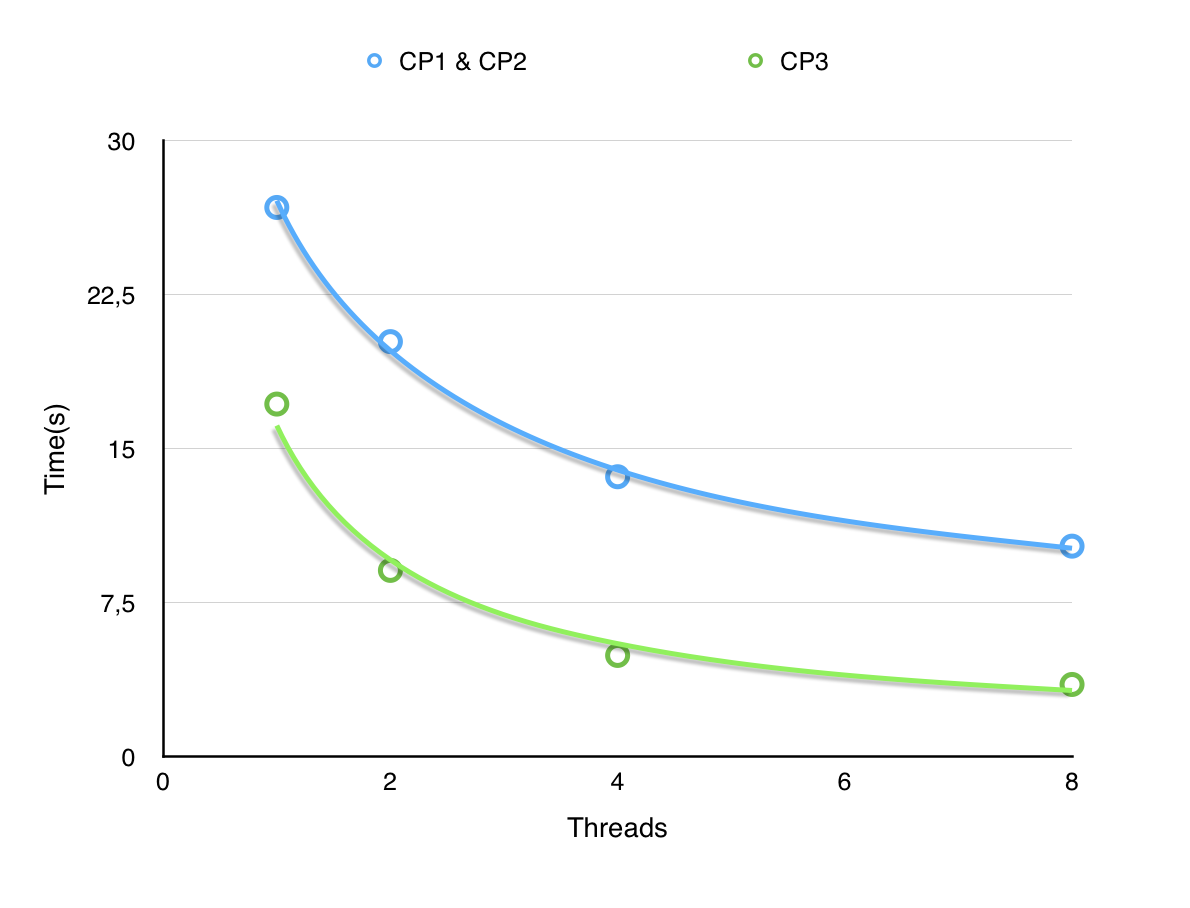
\includegraphics[width=1\textwidth]{figures/w2_time}
\caption{Processing time in a 4000 x 4000 image}
\label{fig:pca_type}
\end{figure}

\begin{figure}[H]
\centering
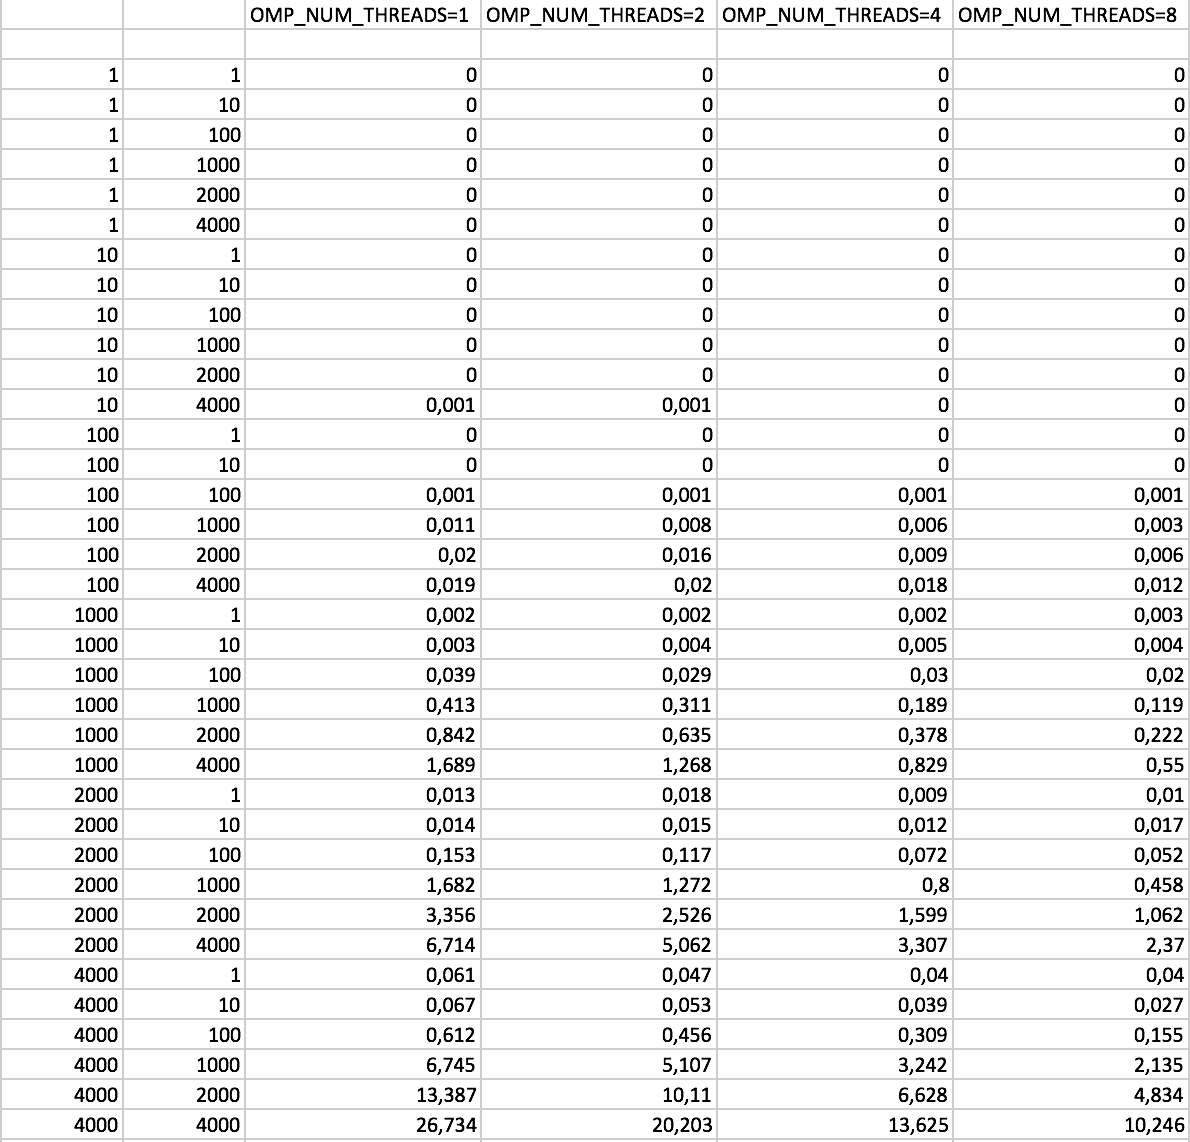
\includegraphics[width=1\textwidth]{figures/w2_cp2}
\caption{CP2 benchmark result}
\label{fig:pca_type}
\end{figure}

\begin{figure}[H]
\centering
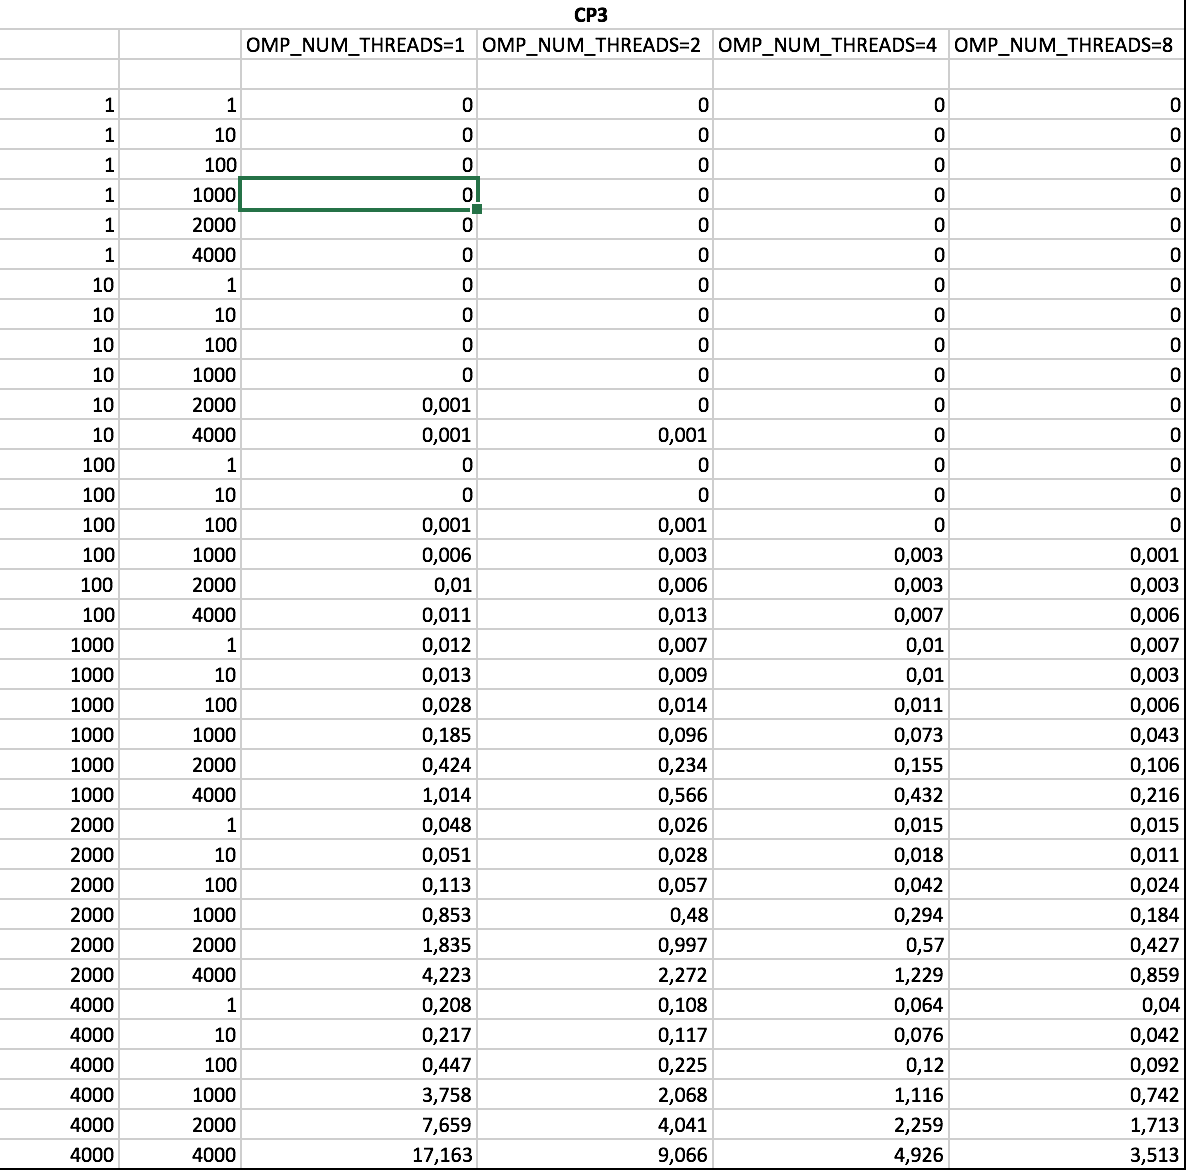
\includegraphics[width=1\textwidth]{figures/w2_cp3}
\caption{CP3 benchmark result}
\label{fig:pca_type}
\end{figure}


I\end{document}